\chapterimage{analisis.jpg} % Table of contents heading image
\chapter{Análisis del sistema e interacción}

La interacción del sistema se puede visualizar mediante diagramas de secuencia, con los cuales se podrá hacer un análisis más clarificado sobre cómo es el ciclo de vida del programa y de qué forma son las relaciones internas de éste.

Para detallar un poco más sobre la comunicación de las partes del sistema, es indispensable un diagrama de comunicación, en donde se podrá detallar los que se transmite entre los objetos, es similar al diagrama de secuencia pero no describe un orden de transmisión de mensajes sino que se centra en los mismos mensajes dados.

Por ultimo, para aclarar cómo se compone el sistema, se explicarán los diagramas de clases, éstos describen cómo están conformadas las calases del sistema, cómo son sus relaciones y sobretodo, cuales son los patrones de diseño que se implementan en la aplicación y cómo optimizan el  funcionamiento de la misma.

%%%%%%%%%%%%%%%%%%%%%% Sección 4.1 %%%%%%%%%%%%%%%%%%%%%%%%%%%
\section{Diagramas de secuencia}

Un diagrama de secuencia muestra una interacción, que representa la secuencia de mensajes entre instancias de clases, componentes, subsistemas o actores. El tiempo fluye por el diagrama y muestra el flujo de control de un participante a otro. Utilice diagramas de secuencia para visualizar instancias y eventos, en lugar de clases y métodos. En el diagrama, puede aparecer más de una instancia del mismo tipo. También puede haber más de una ocurrencia del mismo mensaje \cite{Pw3DS}.

Un diagrama de secuencia es aquel en el que se muestra la interacción entre actores, objetos, interfaces, controles, bases de datos y otras entidades a través del tiempo según el enfoque, el cual puede ser:
\begin{itemize}
	\item \textbf{Enfoque de objetos}: donde son participes las relaciones que existen entre éstos y con actores para realizar una tarea determinada.
	\item \textbf{Enfoque de modelado a tres capas}: donde el actor se comunica con una entidad interfaz, y ésta a su vez con una entidad control para llegar a una persistencia. 
\end{itemize}

Es importante resaltar que cada diagrama de secuencia se realiza en torno a la descripción de un caso de uso dado, ya que éste define el orden en que se deban distribuir las tareas para cada una de las entidades que son participes a la hora de representar cada caso.

Para este proyecto se realizaron 3 casos de uso de los cuales se va a crear un diagrama de secuencia por cada caso y uno para cada enfoque. Inicialmente el caso de uso de REQ-PE (Establecer Panorama) tanto en el enfoque de las tres capas como en el de objetos, igualmente se hará con los dos casos de uso faltantes REQ-ME (Mejora de Estado) y REQ-COM (Comparación Futura) dado que estos incluyen obligatoriamente el anterior.

A continuación se describirá cada diagrama de secuencia:

\paragraph{Diagrama del control de asistencia}

\begin{figure}[H]
	\centering
	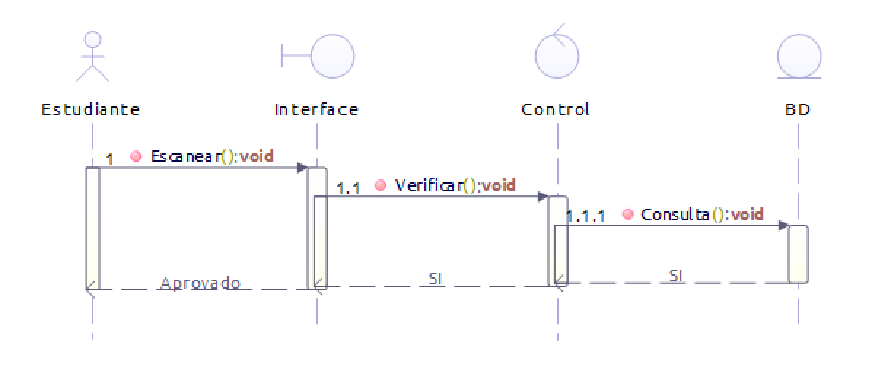
\includegraphics[width=1\linewidth]{parte2/imgs/DiagramaSecuencia/Asistencia}
	\caption[Diagrama de secuencia de registro de Asistencia]{Diagrama de secuencia para el registro del control de asistencia}
	\label{fig:diagramadesecuencia1}
\end{figure}

Las operaciones de los objetos se remiten a guardar y a mostrar una bandera positiva acerca del estado de guardado.

Para establecer el panorama se deben agregar en la base de datos tanto los egresos como los ingresos, pero estos a su vez necesitan ser modificados y/o eliminados conforme pase el tiempo y el estado financiero de la persona cambie, todas estas operaciones se basan en la lectura y/o escritura sobre una base de datos, mientras la interfaz facilita la interacción.

\paragraph{Diagrama del Registro de usuarios}
\begin{figure}[H]
	\centering
	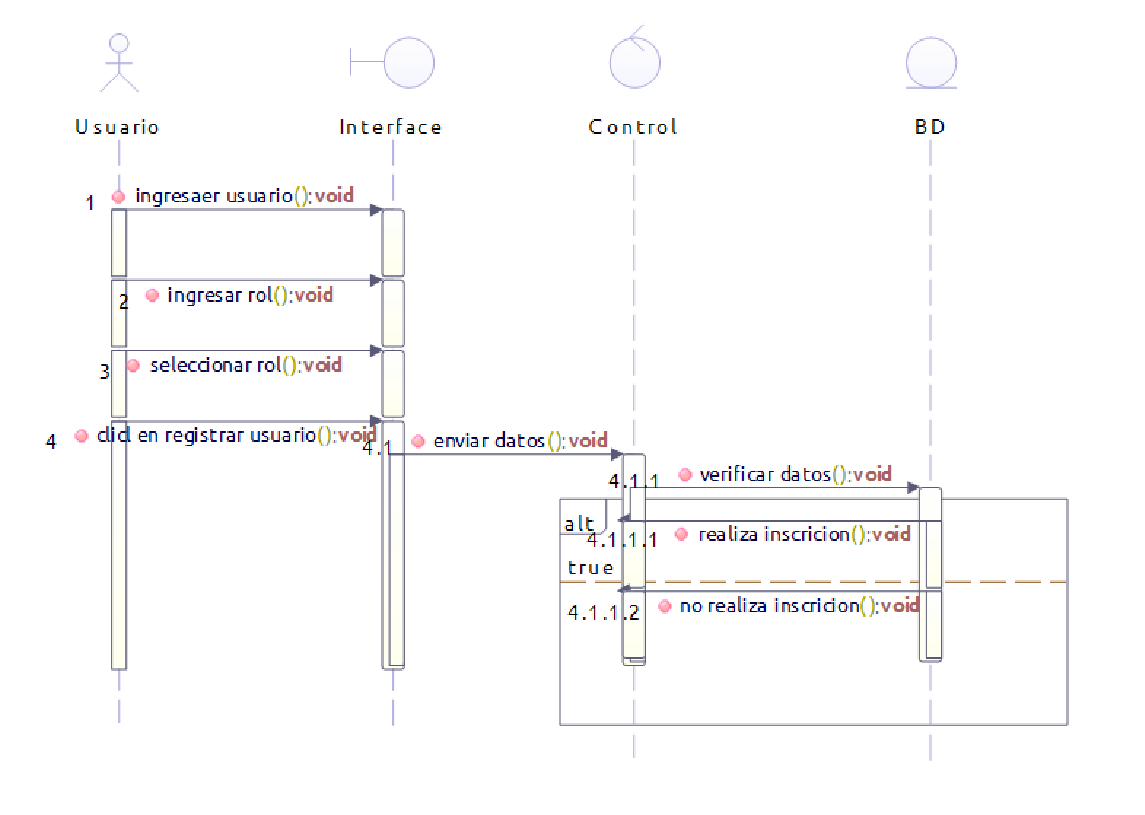
\includegraphics[width=0.8\linewidth]{parte2/imgs/DiagramaSecuencia/RegUsu}
	\caption[Diagrama de secuencia Registrar Usuario]{Diagrama de secuencia para el registro de usuarios}
	\label{fig:diagramadesecuencia2}
\end{figure}

El objeto de sugerencias se encarga de desplegar la lista de sugerencias guardadas en base de datos y da la posibilidad de descartar alguna en específico a criterio del usuario.

Con los primeros datos de ingresos y egresos en base de datos, el programa da unas recomendaciones para un periodo específico acerca de cómo distribuir los ingresos, o en qué cosas se debe invertir más dinero que en otras.

Conforme se van agregando datos y acumulando sugerencias, se da la posibilidad de que la aplicación muestre proyecciones acerca de un estado futuro comparan un futuro y otro donde se ubique un futuro donde se haga caso a una o más sugerencias del programa.

Listar las sugerencias no descartadas de base de datos para alimentar las proyecciones, y sobre ésta lista permitir seleccionar cuales sugerencias quiere proyectar y cuales descartar

\paragraph{Diagrama para crear nuevas convocatorias}
\begin{figure}[H]
	\centering
	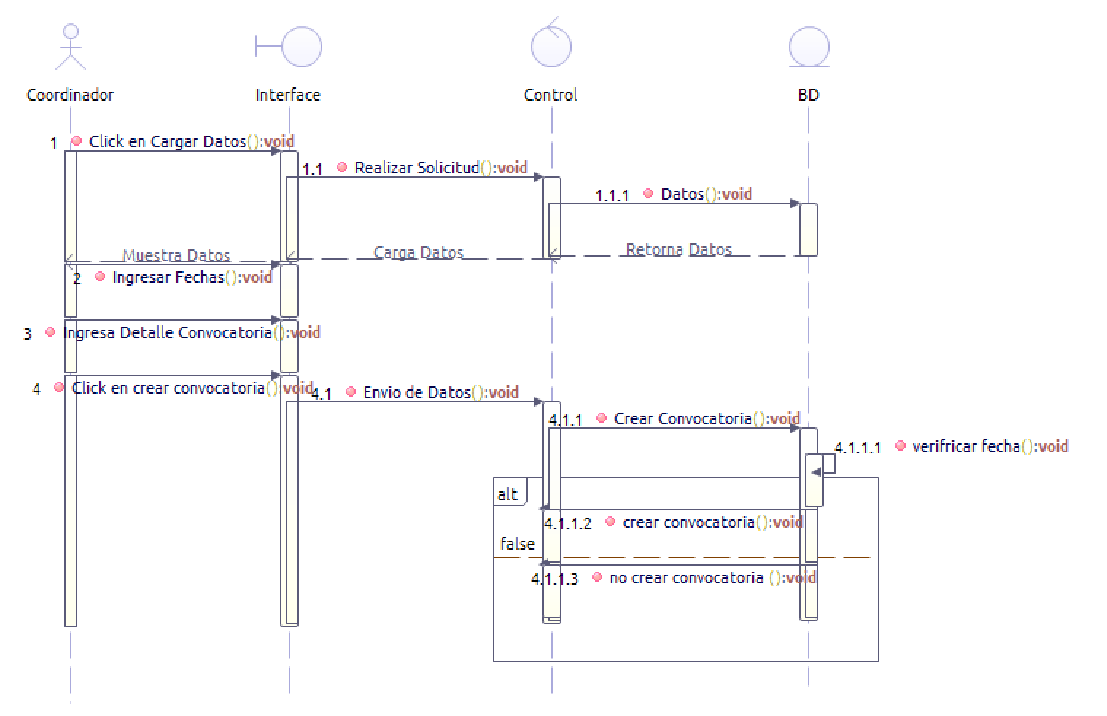
\includegraphics[width=0.8\linewidth]{parte2/imgs/DiagramaSecuencia/SecCrearConv}
	\caption[Diagrama de secuencia Crear convocatoria]{Diagrama de secuencia para crear una nueva convocatoria}
	\label{fig:diagramadesecuencia5}
\end{figure}

Las comparaciones dadas por el programa se dan a partir del flujo de ingresos y egresos dados por el usuario, versus las sugerencias dadas por la aplicación, posteriormente, después de que el usuario seleccione una o mas posibilidades arrojadas por el programa este genera gráficas de estimaciones acerca de como estaría su situación económico haciendo caso de las sugerencias del programa sobre su situación actual y las contrasta con un proyección en donde no cambia ninguna recomendación. 

\paragraph{Diagrama del registro a convocatoria existentes}
\begin{figure}[H]
	\centering
	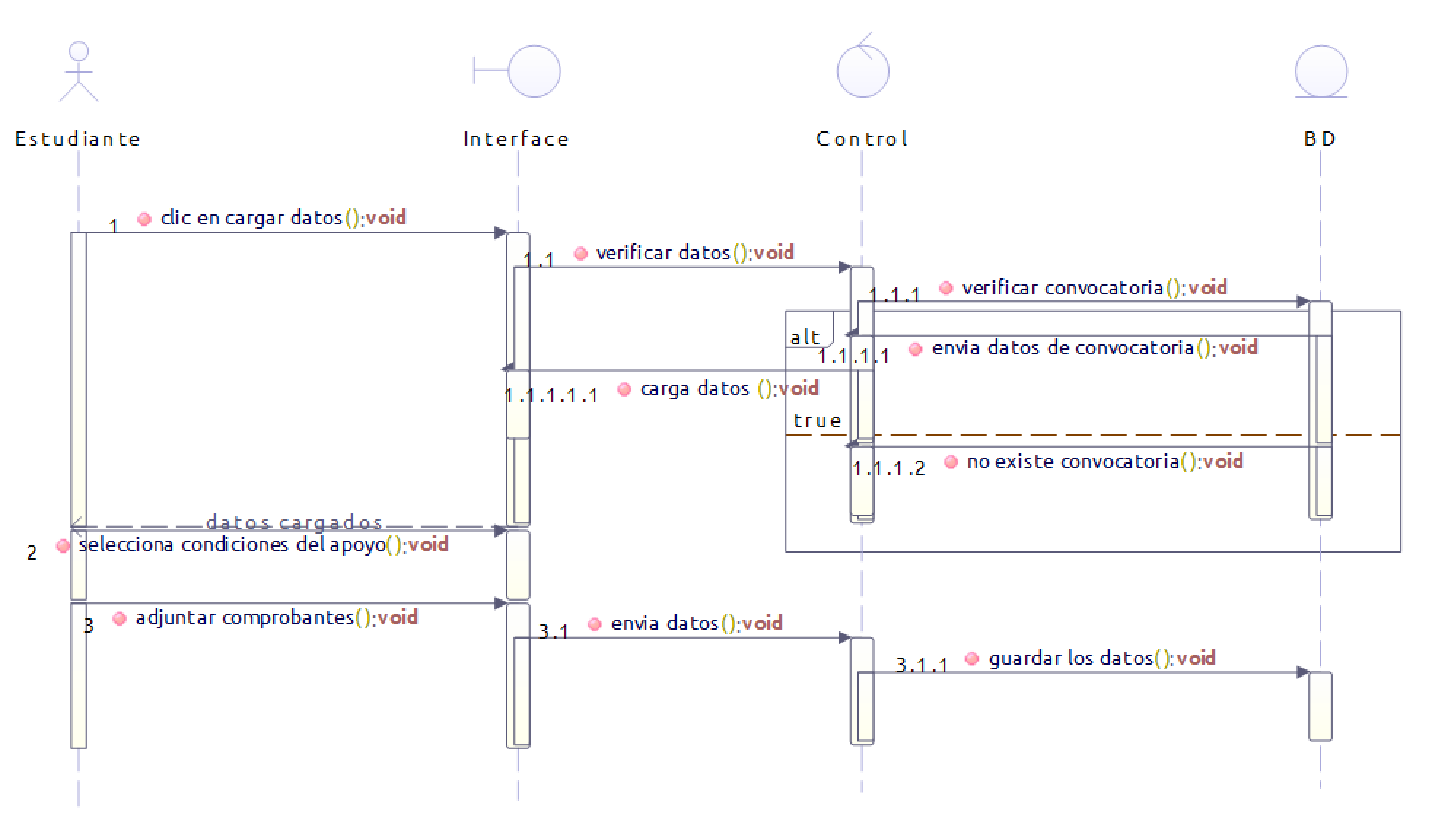
\includegraphics[width=0.8\linewidth]{parte2/imgs/DiagramaSecuencia/SecSolConv}
	\caption[Diagrama de secuencia Registro a una convocatoria]{Diagrama de secuencia para el registro a una convocatoria}
	\label{fig:diagramadesecuencia3}
\end{figure}
Básicamente, para el diagrama de secuencia enfocado a objetos, el caso de uso REQ-EP solo necesita entrada de datos (tanto para egresos como para ingresos) que son los que permiten que la aplicación empiece un trabajo de background de análisis y desarrollo de sugerencias para el usuario.

\paragraph{Diagrama de la verificacion de una solicitud a una convocatoria}
\begin{figure}[H]
	\centering
	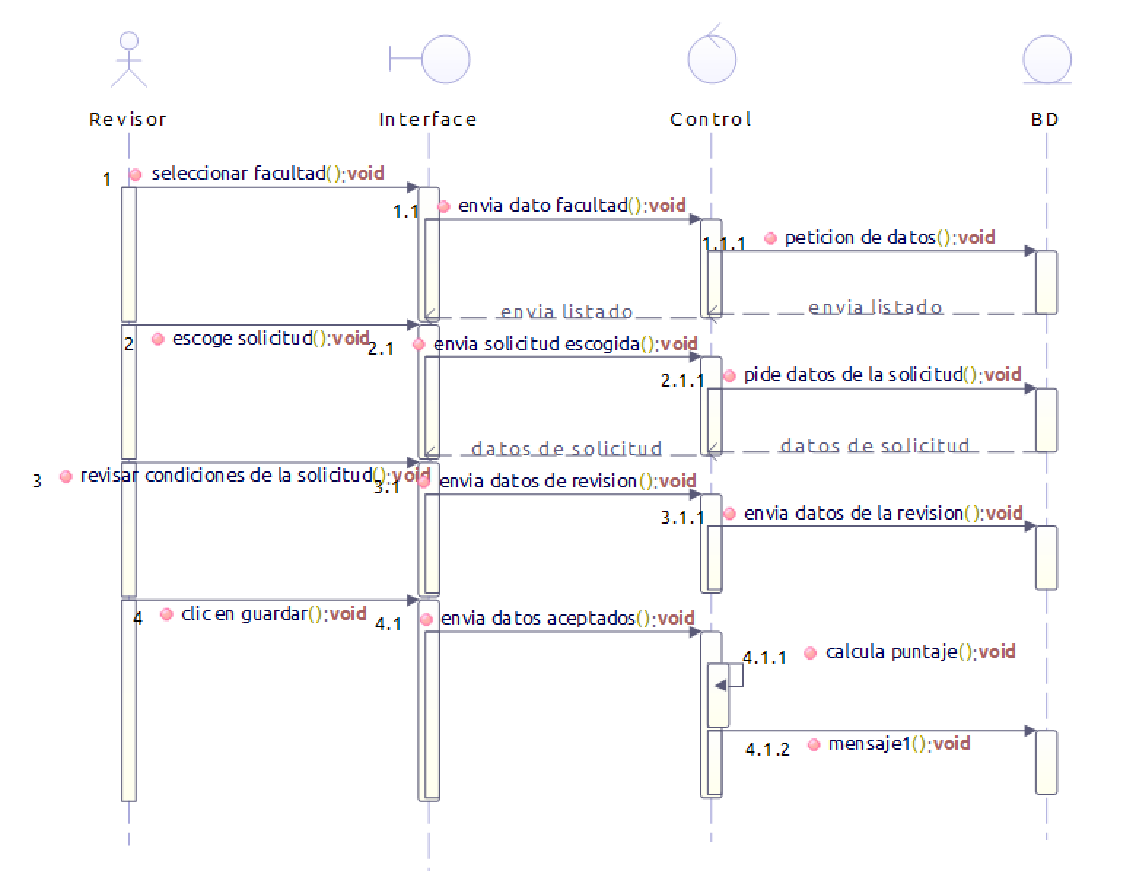
\includegraphics[width=0.8\linewidth]{parte2/imgs/DiagramaSecuencia/SecVerifSolConv}
	\caption[Diagrama de secuencia Verificacion de solicitud]{Diagrama de secuencia de verificacion de una solicitud a una convocatoria}
	\label{fig:diagramadesecuencia4}
\end{figure}

Para la muestra de sugerencias, el objeto debe proveer la forma de visualizarlas para el usuario, por lo cual este lanza el mensaje de ver sugerencia, y dentro de la lista desplegada, el usuario puede descartar alguna sugerencia en especifico a criterio personal, por lo cual este es un mensaje del objeto a si mismo.

\newpage

%%%%%%%%%%%%%%%%%%%%%% Sección 4.2 %%%%%%%%%%%%%%%%%%%%%%%%%%%
\section{Diagramas de comunicación}

También llamados Diagramas de Colaboración. Nos sirven para enfatizar los vínculos de datos entre los participantes de una interacción. Un diagrama de Comunicación modela las interacciones entre objetos o partes en términos de mensajes en secuencia. Los diagramas de Comunicación representan una combinación de información tomada desde el diagrama de Clases, Secuencia, y Diagrama de casos de uso describiendo tanto la estructura estática como el comportamiento dinámico de un sistema \cite{Pw4DC}.

Los diagramas de comunicación tienen la función de simplificar la visualización de los modelos, dado que se enfocan exclusivamente en los objetos y su interacción, la cual se hace por medio de mensajes. Para seguir la lectura de un diagrama de comunicación se procede a ubicar el mensaje con la enumeración de primer orden, y se sigue la dirección indicada por la flecha adjunta, y así sucesivamente hasta llegar al último mensaje. Este tipo de diagrama se encuentra muy relacionado con el diagrama de secuencia, dado un isomorfismo entre éstos; Son equivalentes, pero tienen dos puntos de vista.


\paragraph{Diagrama del control de asistencia}
\begin{figure}[H]
	\centering
	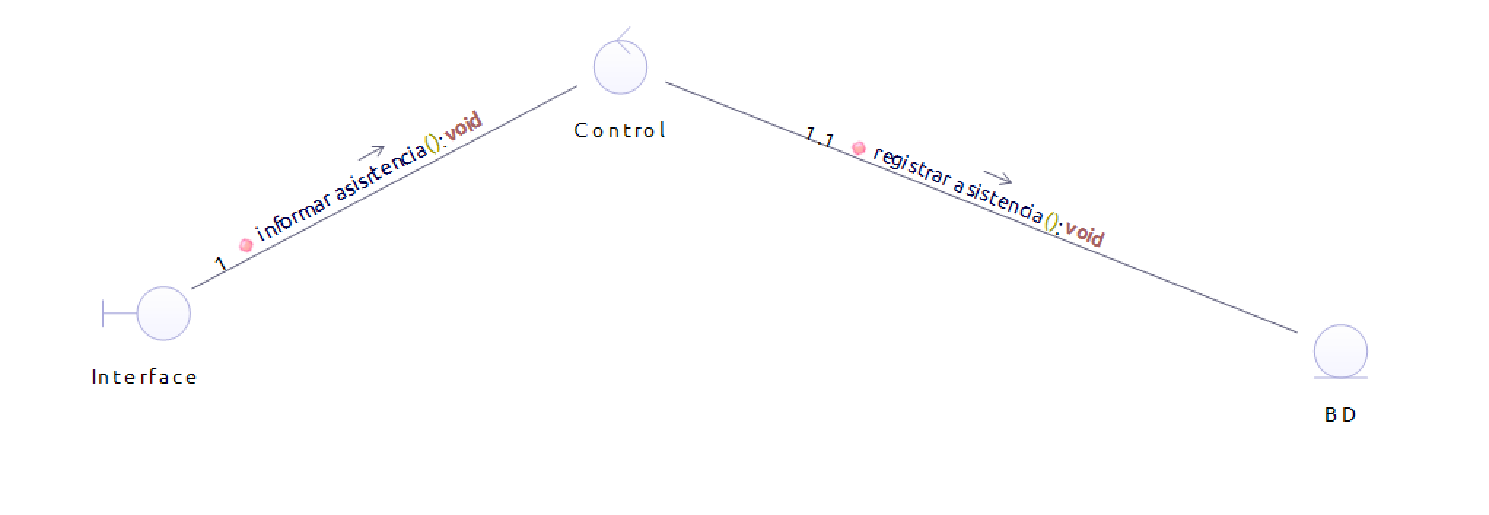
\includegraphics[width=1\linewidth]{parte2/imgs/DiagramaComunicacion/ComAsist}
	\caption[Diagrama de Comunicacion Control de asistencia]{Diagrama de Comunicación del control de asistencia}
	\label{fig:diagramaDeComunicacion}
\end{figure}

En el diagrama de la figura 4.7 se tiene que el usuario invoca la vista general de los ingresos y egresos, y es desde la cual agrega un nuevo ingreso al enviar el mensaje de "nuevoIngresoOEgreso", que se encarga de llamar a la base de datos por medio del método "guardarRegistro" y en tanto, y al momento de realizarse este la lista invoca otro método de la vista encargado de actualizar la lista de mensajes que también llama a la base de datos mediante el mensaje "leerRegistros".\newline%newpage para machetear y que no se vea tan paila

\paragraph{Diagrama del registrode usuarios}
\begin{figure}[H]
	\centering
	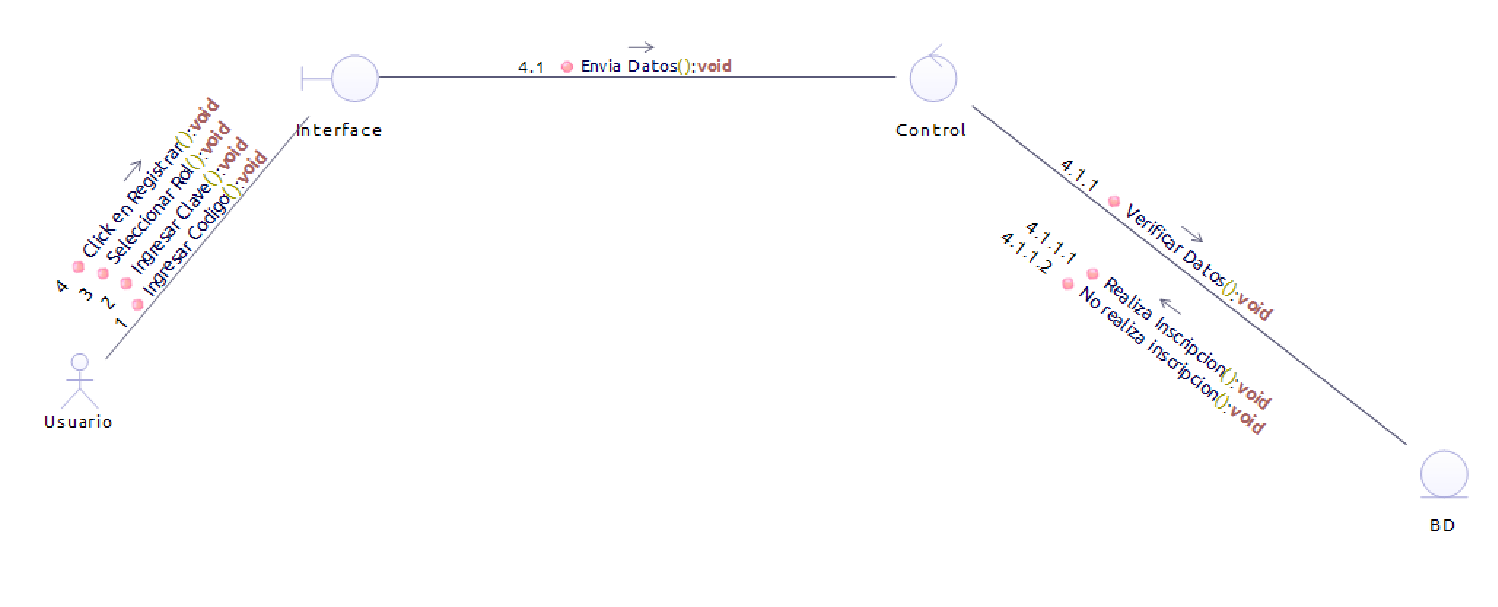
\includegraphics[width=1\linewidth]{parte2/imgs/DiagramaComunicacion/ComReguU}
	\caption[Diagrama de Comunicacion del registro de usuarios]{Diagrama de Comunicación del registro de usuarios}
	\label{fig:diagramaDeComunicacion3}
\end{figure}

Para la comunicación entre el usuario y el objeto de sugerencias se usa el mensaje "verSugerencias" y en donde el objeto de sugerencias provee la forma de eliminar sugerencias usando el mensaje "descartarSugerencia"

\paragraph{Diagrama de la creacion de una convocatoria}
\begin{figure}[H]
	\centering
	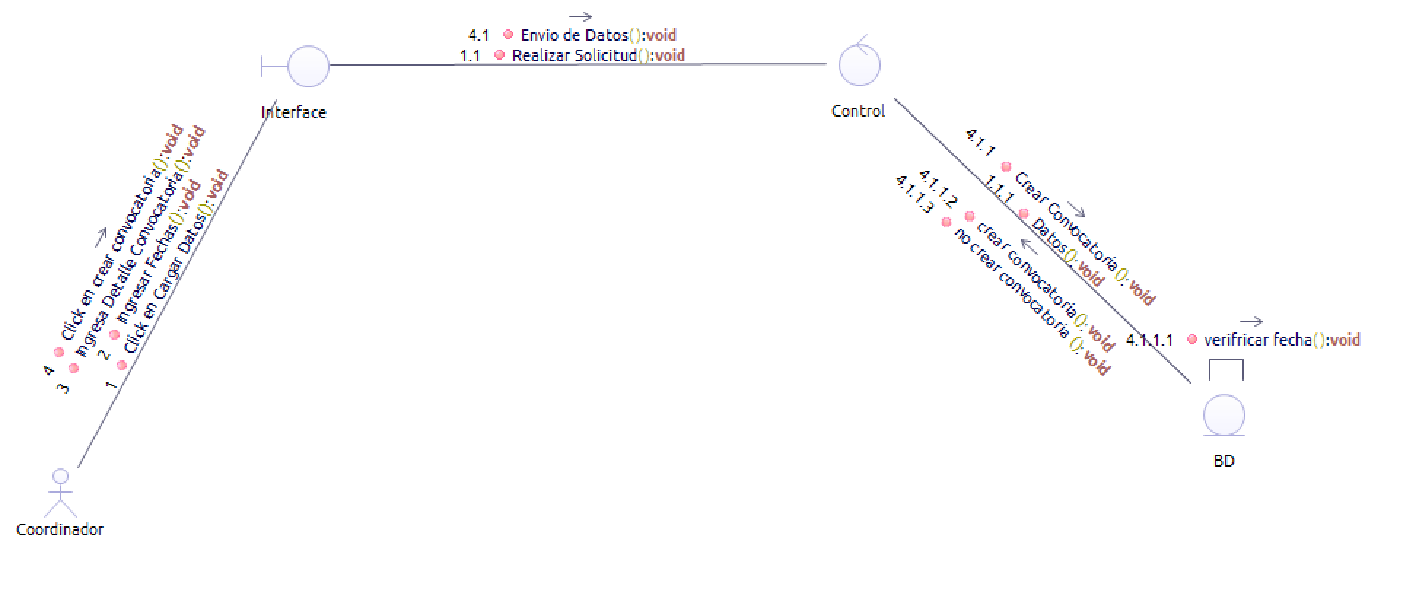
\includegraphics[width=1\linewidth]{parte2/imgs/DiagramaComunicacion/ComCreConv}
	\caption[Diagrama de Comunicacion cfracion Covoactoria]{Diagrama de Comunicación de la creacion de una convocatoria}
	\label{fig:diagramaDeComunicacion5}
\end{figure}

En el diagrama 4.9 vemos la relación que existe entre el usuario con la aplicación para ver la comparativa de su estado económico actual con el posible estado económico que puede tener al seguir rigurosamente las sugerencias que le brinda la aplicación, si nos guiamos por las flechas del diagrama vemos como el actor le pide a la interfaz de comparaciones el método "mostrarComparativa" en dónde se le mostrará al usuario dicha comparación traida del control usando el método "leerComparaciones", las cuales se desarrollan a través del proceso de datos tanto del usuario como de los tentativos datos de mejoras que podemos encontrar en nuestra base de datos, para ello utilizamos el método "leerDatos" y con esto estaría terminado la forma en que se comunican las entidades de la aplicación destinadas a cumplir este caso de uso.

\paragraph{Diagrama para la solicitud a una convocatoria}
\begin{figure}[H]
	\centering
	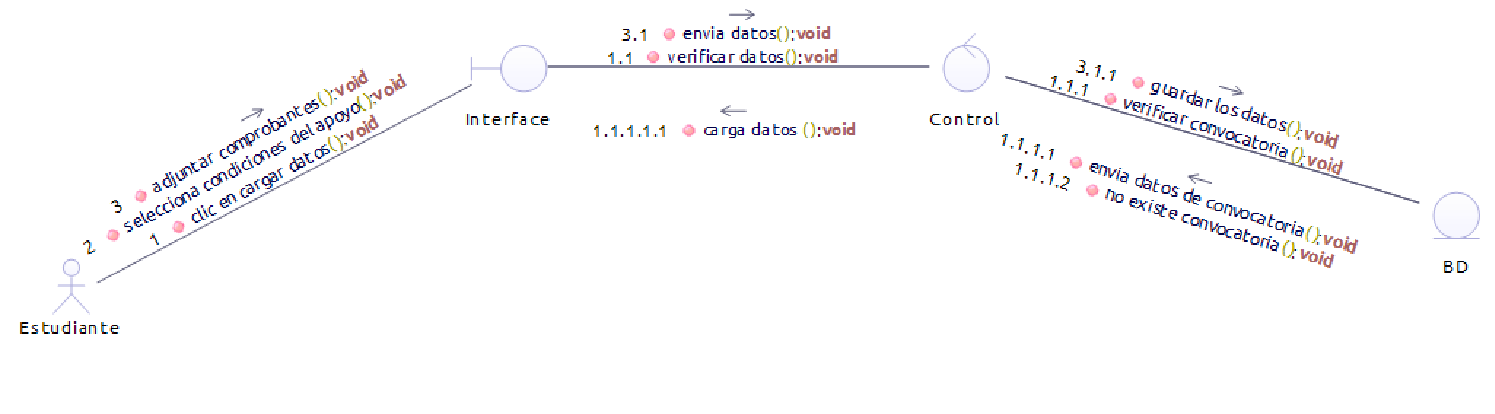
\includegraphics[width=1\linewidth]{parte2/imgs/DiagramaComunicacion/ComSoliConv}
	\caption[Diagrama de Comunicacion Solicitud a Convocatoria]{Diagrama de Comunicación para la solicitud a una convocatoria}
	\label{fig:diagramaDeComunicacion2}
\end{figure}

Para la figura 4.10 se puede ver la independencia de los procesos de inserción de egreso e ingreso, en donde los objetos respectivos se encargan de guardarlo.

\paragraph{Diagrama de la verificacion de una solicitud}
\begin{figure}[H]
	\centering
	\includegraphics[width=1\linewidth]{parte2/imgs/DiagramaComunicacion/Comver}
	\caption[Diagrama de Comunicacion verificacion solicitud]{Diagrama de Comunicación de la  verificacion de una solicitud}
	\label{fig:diagramaDeComunicacion4}
\end{figure}

La interacción entre el usuario y la lista de sugerencias no se realiza a través de mensajes, pero para descartar sugerencias se realizan mediante el mensaje "descartarSugerencias" que se encarga de llamar a la base de datos mediante "eliminarSugerencia" para borrar una sugerencia en la base de datos, y se vuelve a cargar los datos para actualizar la lista de sugerencias es la vista.

\newpage

%%%%%%%%%%%%%%%%%%%%%% Sección 4.3 %%%%%%%%%%%%%%%%%%%%%%%%%%%
\section{Diagramas de clases}

Para una análisis orientado al desarrollo del aplicativo se plantean los diagramas de clases, que básicamente representa la interacción entre distintas entidades que en conjunto logran cumplir con la funcionalidad del programa. Los diagramas de clases se componen principalmente de:

\begin{itemize}
	\item  \textbf{Clase}: Esta es la entidad que representara un objeto que interviene en la solución del problema. Su ilustración es un rectángulo dividido en 3 niveles: En el primero esta el nombre, el segundo es para los atributos y el ultimo es para las operaciones de dicho objeto
	\item \textbf{Relación}: Las relaciones se encargan de mostrar como es la interacción entre las clases de un diagrama, permite la comunicación entre las mismas y se dividen en 4 fundamentalmente
	\begin{itemize}
		\item \textit{\textbf{Herencia}}: Se encuentra en las clases cuando una clase "es una" clase aparte ya definida, en donde la herencia permite realizar una especialización, o en sentido inverso, hacer una generalización de unas características o comportamientos.
		\item \textit{\textbf{Dependencia}}: Se da cuando una clase depende de otra para su existencia o uso, pero la existencia de la primera no interfiere en la existencia de la segunda.
		\item \textit{\textbf{Asociación}}: Ocurre cuando una clase puede usar otra sin que sea obligatorio inicializarla al iniciar la clase principal
		\item \textit{\textbf{Composición}}: Es parecida a la asociación, sin embargo, esta relación hace obligatoria la inicialización de la clase agregada al momento de usar la clase principal.
	\end{itemize}
\end{itemize}

Haciendo uso de las clases y relaciones en un diagrama se puede llegar a una solución para el problema en un momento especifico en el tiempo, pero hay que tener en cuenta que el software debe poder perdurar en el tiempo de forma limpia, sin necesidad de hacer cambios como tal en el código existente sino solo permitir la adición de componentes o clases, para ello se usan los patrones de diseño que no son mas sino estructuras de clases y relaciones enfocadas solucionar los problemas del mantenimiento del software, mejorando así el ciclo de vida de la aplicación.

En los siguientes diagramas se mostraran algunos patrones de diseño en nuestra aplicación enfocados a distintos problemas al momento de plasmar la aplicación en un diagrama de clases.

\subsection{Creacionales}

\paragraph{Builder}
\begin{figure}[H]
	\centering
	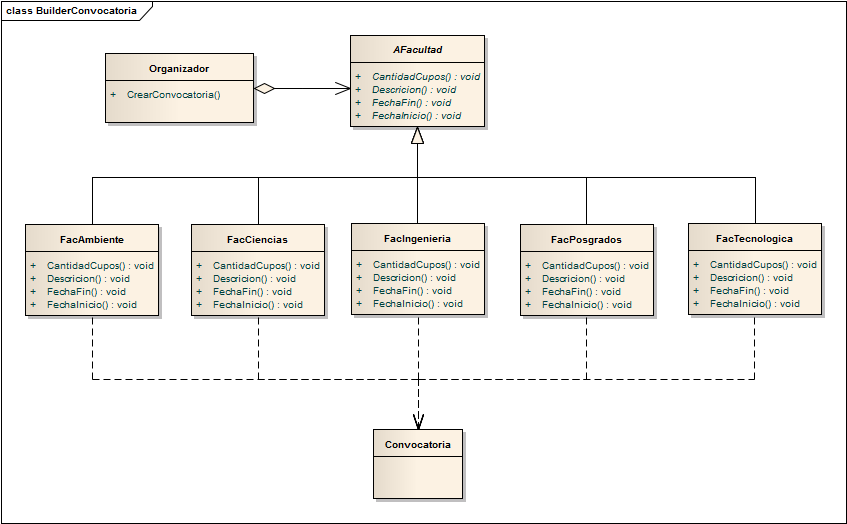
\includegraphics[width=1\linewidth]{parte2/imgs/Patrones/BuilderConvocatoria}
	\caption[Diagrama de clases del patrón Builder]{Diagrama de Clase para creación de de convocatorias por facultad}
	\label{fig:fabricaAbstracta}
\end{figure}

El patrón de diseño Abstract Factory permite agrupar la creación de objetos mediante una interfaz de creación compartida por fabricas que se especializan en crear los objetos de un grupo especifico. Este patrón nos sirve para la creación de sugerencias y flujos económicos ya que estos comparten atributos y una interfaz de comportamiento, por lo que las fabricas solo deben ocuparse de construir objetos de algún tipo de objeto que es o egreso o ingreso.

\paragraph{Factory}
\begin{figure}[H]
	\centering
	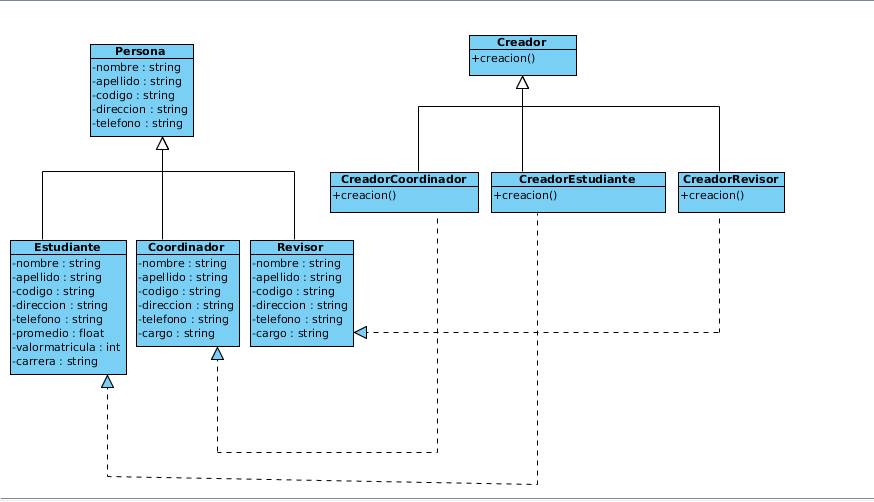
\includegraphics[width=1\linewidth]{parte2/imgs/Patrones/FactoryMethod}
	\caption[Diagrama de clases del patrón Facade]{Diagrama de Clase para el manejo de la conexión a distintas bases de datos a través del patrón de diseño Facade}
	\label{fig:facade}
\end{figure}

El patrón de diseño Facade se encarga principalmente es de encapsular la complejidad de un modulo y permitir el acceso a este solo a través de una fachada, que se provee por medio de una interfaz para que otros módulos puedan consumir los servicios del modulo sin que se enfrenten a la complejidad del mismo. Se selecciono éste para la gestión de las conexiones a la base de datos ya que cada motor ofrece una forma distinta de consumo de servicios, ademas de distintos controladores con los que trabajar, por lo que es mas sencillo encerrar todas esas clases dentro de un solo modulo y proveer una interfaz estandarizada para hacer uso de la conexión

\paragraph{Singleton}
\begin{figure}[H]
	\centering
	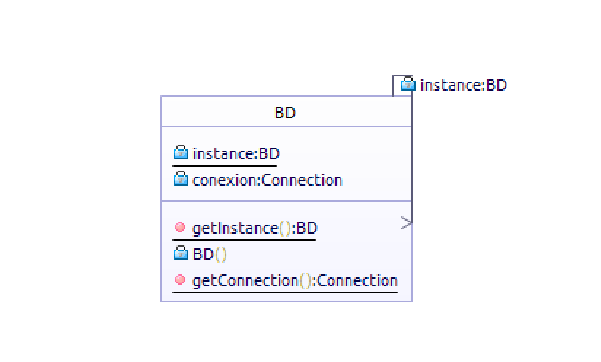
\includegraphics[width=1\linewidth]{parte2/imgs/Patrones/Singleton}
	\caption[Diagrama de clases del patrón Singleton]{Diagrama de Clase para el manejo de las operaciones de escritura/lectura sobre base de datos a través del patrón de diseño Bridge}
	\label{fig:puente}
\end{figure}

El patrón de diseño Bridge permite separar comportamientos diferentes usando una interfaz, y al momento de ejecutarse el metodo de la interfaz, sea cual sea el comportamiento seleccionado, este se ejecuta sin necesidad de que quienes lo invoquen sepan que contiene realmente. Este patrón resulta útil al momento de realizar operaciones sobre la base de datos ya que elimina la necesidad de saber que base de datos se esta usando en cierto momento, y solo ejecuta el llamado del método de la interfaz para efectuar cierta operación en especifico.

\subsection{Comportamiento}

\paragraph{Iterador}
\begin{figure}[H]
	\centering
	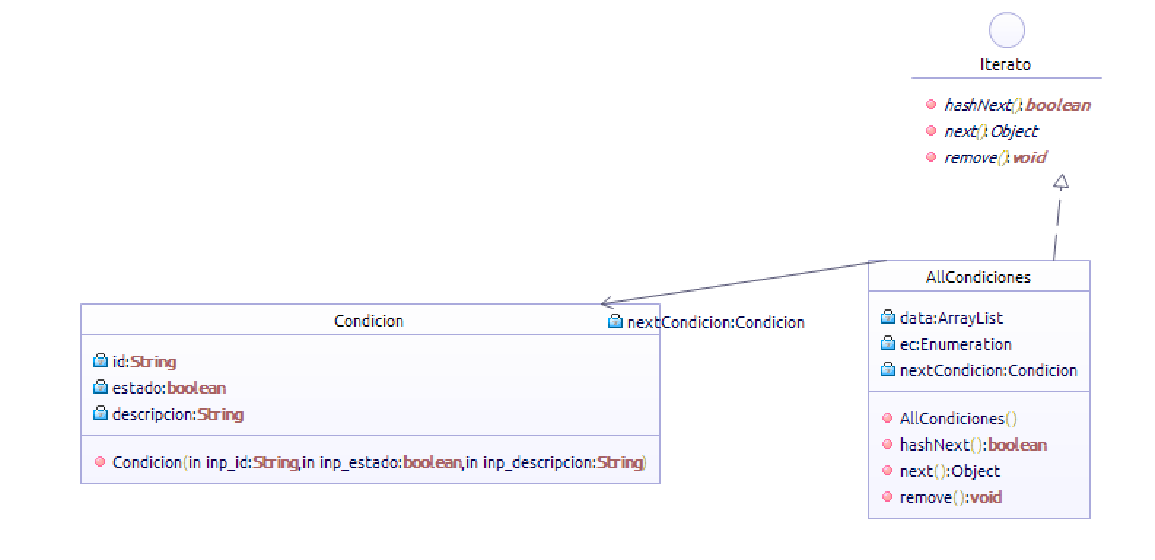
\includegraphics[width=1\linewidth]{parte2/imgs/Patrones/Iterador}
	\caption[Diagrama de clases del patrón Command]{Diagrama de Clase para la ejecucion de acciones de CRUD mediante el patron de diseño Comando}
	\label{fig:command}
\end{figure}

El patrón de diseño Command se concibe como un ejecutor de funciones, haciendo que cada clase que implementa la interfaz command tenga dentro de si el objeto que debe ejecutar la función, pero sin conocer puntualmente cual es. Para la realización de operaciones CRUD (Create-Read-Update-Delete) desde los servicios el command se encarga de llamar en cada command concreto una función crud en particular, sin conocer cual es su contenido sino simplemente lanzando su ejecución

\paragraph{State}
\begin{figure}[H]
	\centering
	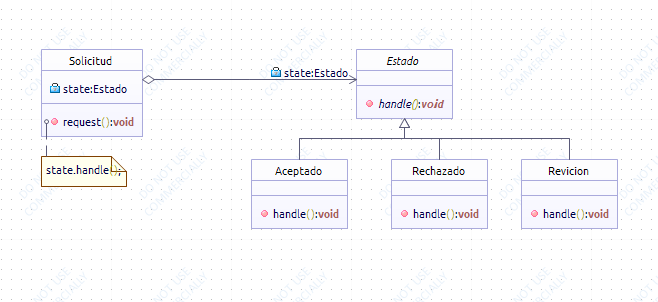
\includegraphics[width=1\linewidth]{parte2/imgs/Patrones/Estado}
	\caption[Diagrama de clases del patrón Mediator]{Diagrama de Clase para la relacion entre flujos financieros y sugerencias mediante el patron de diseño Mediator}
	\label{fig:mediador}
\end{figure}

El patrón de diseño Mediator encapsula la interacción entre dos o mas clases sin hacer que estas se traten directamente. Para relacionar sugerencias y flujos económicos resulta útil para evitar el acoplamiento entre ellos al relacionar, por ejemplo, que flujos interfieren en una sugerencia especifica, o también en cuantas sugerencias interviene un mismo flujo.

